%% LyX 2.0.0 created this file.  For more info, see http://www.lyx.org/.
%% Do not edit unless you really know what you are doing.
\documentclass[english]{article}
\usepackage[T1]{fontenc}
\usepackage[latin1]{inputenc}
\usepackage{units}
\usepackage{textcomp}
\usepackage{amsmath}
\usepackage{graphicx}
\usepackage{esint}

\makeatletter
%%%%%%%%%%%%%%%%%%%%%%%%%%%%%% User specified LaTeX commands.
%\usepackage{geometry}
%
\usepackage{graphics}\usepackage{a4wide}

\usepackage{babel}

\makeatother

\usepackage{babel}
\begin{document}

\title{The Solvation Effect (Continuum Model) into ParaGauss}


\author{Shor A. M.}

\maketitle

\section{Introduction}

Current efforts in solvation modeling in general follow one of the
following two approaches. The first one involves the explicit consideration
of hundreds or thousands of solvent molecules. The supermolecular
system consisting of solvent molecules plus the solute molecule serve
as basis for simulations from which solvation related thermodynamic
data may be extracted. A molecular mechanics force field is employed
in general, since huge size of the system makes the analysis of forces
and energies at the quantum mechanical level difficult, although combinations
of quantum mechanical treatment of the solute with a molecular mechanical
one of the solvent molecule is also very popular.

The alternative simulation procedure is to replace the explicit solvent
molecules by a continuous medium with the dielectric constant of the
bulk. Once the solvent has been simplified, it is possible to apply
quantum mechanical methods to describe the solute within the solvent
\cite{Cramer95}. The continuous descriptions must be well tailored
on the characteristics of the specific case under examination, with
appropriate tuning of all elements of the model. The interaction between
solute and solvent is described by means the effective Hamiltonian
which consists of the molecular Hamiltonian $H^{0}$ and the interaction
potential $V_{R}$ \cite{Tomasi99}.

The interaction between two systems (solute and solvent) includes
different terms: the electrostatic contribution, dispersion term,
repulsion term and so on. The most important component of $V_{R}$
is the electrostatic interaction $V_{el}$ between the solute molecule
$M$ and the solvent in which it is embedded (especially for polar
system). This component is defined by considering the dielectric properties
of the continuous solvent. The simplest and most exploited model describes
the solvent as a continuous Isotropic distribution with Linear Dielectric
response (ILD model \cite{Tomasi99}).

There are many ways to solve the ILD solvation problem, but the most
successful of them is the combination of an irregular cavity of a
molecular shape and the use of Apparent Surface Charges (ASC) which
reduces the solution of combined Poisson 
\begin{equation}
\Delta V(r)=-4\pi\rho\quad r\in{\mathrm{i}nside\: cavity}\label{int1}
\end{equation}
 and Laplace 
\begin{equation}
\Delta V(r)=0\quad r\in{\mathrm{o}utside\: cavity}\label{int2}
\end{equation}
 equations to a two dimensional integral equations on a close surface
(molecular cavity), in general solved with the aid of the Boundary
Element Method (BEM).

The ASC formulation was first employed at QM level in 1981\cite{Miertus81}
as the Polarizable Continuum Model (PCM). In the beginning the PCM
approach only dealt with the electrostatic problem of the solvation
effect and treated only isotropic solvents. But later PCM was rapidly
extended to the other liquid systems (anisotropic dielectric\cite{Mennucci95},
non-homogeneous description of the solvent\cite{Cossi94}) and to
a large set of properties (dispersion-repulsion contribution to free
solvation energy \cite{Floris91,Amovili94,Amovili97}, analytical
derivatives for molecular solutes with respect to nuclear coordinates
and other external parameters\cite{Cammi94,Cammi94a}).

In 1993 Klamt and Sch��rmann suggested a new model which describes
the reaction field of the continuous solvent using a screening conductor
theory\cite{Klamt93}. This model had been called COSMO (COnductor
like Solvation Model). The COSMO approach describes the apparent polarization
charges distributed on the cavity surface by supposing that the total
electrostatic potential vanishes at the cavity boundary. The first
implementation of COSMO model was done on semi-empirical level\cite{Klamt93}
and later extended to an ab initio level \cite{Stefan95,Klamt95,Barone98}.
The COSMO was the first among the family of PCM methods which had
refused to use the iterative procedure to calculate the point charges
spread on the cavity surface and adopted a new matrix inversion procedure.
This step allowed to include a calculation of the solvent reaction
field directly in the SCF procedure. That is, the solute electron
density and reaction field are converged simultaneously. In this case
the time spent to carry out quantum chemical calculations reduces
significantly.


\section{Basic aspects of the PCM (polarizable continuum model) procedure}

The system under consideration in the PCM approach is the solute molecule
$M$ located inside the cavity of molecular shape surrounded by an
infinite continuous solvent. According to Ben-Naim\cite{Ben-Naim87},
the solvation process of the solute \emph{M} in solvent consists of
transferring \emph{M} from a fixed position in the ideal gaseous phase
to a fixed position in a solvent, at constant temperature \emph{T},
pressure \emph{P} and chemical composition. The Gibbs free energy
of solvation can be related to the work necessary to assemble solute
\emph{M} in a solvent, \emph{W}. There is a connection between \emph{W}
and the measurable free energy change. The following expression may
be accepted as good approximation to the solvation free energy: 
\begin{equation}
\Delta G_{sol}=W+RT\ln\left(\frac{q_{rot,g}q_{vib,g}}{q_{rot,s}q_{vib,s}}\right)-RT\ln\left(\frac{n_{M,g}\Lambda_{M,g}^{3}}{n_{M,s}\Lambda_{M,s}^{3}}\right)\label{pcm1}
\end{equation}
 Here $q_{rot,g}$, $q_{vib,g}$, $q_{rot,s}$, $q_{vib,s}$ are the
microscopic partition functions for rotation and vibration of \emph{M},
in gas phase and in solution; $n_{M,g}$, $n_{M,s}$ are numerical
densities of \emph{M} molecules; $\Lambda_{M,g}^{3}$, $\Lambda_{M,s}^{3}$
are the momentum partition functions \cite{Tomasi94}. There is additional
term , $P\Delta V$, but it can be neglected because of its value
is usually less then $10^{-3}$ Kcal/mol. The last two parts in eq.
(\ref{pcm1}) are known as the molecular motion (\emph{Mm}) contribution
to the solvation free energy. One can introduce a partition of the
work \emph{W} into electrostatic (\emph{el}), repulsion (\emph{rep}),
dispersion (\emph{dis}) and cavitation (\emph{cav}) (the work spent
to build the cavity with the appropriate shape inside the solvent)
contributions: 
\begin{equation}
W=\Delta G_{el}+G_{rep}+G_{dis}+G_{cav}\label{pcm2}
\end{equation}


Then we can present the solvation free energy as: 
\begin{equation}
\Delta G_{sol}=\Delta G_{el}+G_{rep}+G_{dis}+G_{cav}+\Delta G_{Mm}\label{pcm3}
\end{equation}


The use of the symbol $\Delta$ emphasizes the fact that the first
and last terms of $\Delta G_{sol}$ are defined as differences of
two independent calculations: the solute in solution and the solute
in vacuum.

The quantum mechanical problem of the treatment of the continuous
solvation model can be expressed by the following Schr�dinger equation
\begin{equation}
(H^{0}+V_{R})\Phi=E\Phi\label{pcm4}
\end{equation}
 where $H^{0}$ is the Hamiltonian of the solute in vacuum, $V_{R}$
is the interaction potential between solute and solvent, $\Phi$ is
the wave function of the solute.

In parallel to the free energy, the interaction potential $V_{R}$
can be decomposed to: 
\begin{equation}
V_{R}=V_{el}+V_{dis}+V_{rep}\label{pcm5}
\end{equation}


In principle $V_{R}$ is functionally depending on the charge distribution
of the solute \emph{M 
\begin{equation}
V_{R}=V_{R}\left[\rho_{M}\right]\qquad,\label{pcm6}
\end{equation}
 } and therefore it is conveniently to separate $V_{R}$ into two
components which are dependent and independent of the charge distribution
of \emph{M 
\begin{equation}
V_{R}=V_{R}^{\prime}\left[\rho_{M}\right]+V_{R}^{\prime\prime}\label{pcm7}
\end{equation}
 }

According to the basic principles of quantum mechanics the variational
solution of the Schr�dinger equation requires the minimization of
a functional $J^{S}$ which has the status of a free energy 
\begin{equation}
J^{S}=\left\langle \mu\right|H^{0}+V_{R}^{\prime\prime}+\frac{1}{2}V_{R}^{\prime}\left[\rho_{M}\right]\left|\nu\right\rangle \label{pcm8}
\end{equation}
 where $\Psi$ is the trial wave function.

The minimization of the free energy functional $J^{S}$ can be reduced
to a matrix equation 
\begin{eqnarray}
H^{\prime}C & = & SC\varepsilon\nonumber \\
\mathrm{with}\nonumber \\
H^{\prime} & = & h^{\prime}+G^{\prime}\left(P\right)\label{pcm9}
\end{eqnarray}
 where \emph{C}, \emph{S} and $\varepsilon$ represent the standard
matrices of the molecular orbital coefficients, of the overlap and
of the one-electron orbital energy, exactly as in vacuo. The matrix
$H^{\prime}$ is modified with respect to calculation in vacuo and
it is separated into an one-electron term ($h^{\prime}$) and a two-electron
term ($G^{\prime}(P)$) \cite{Cossi95}.

We can limit ourselves considering only the electrostatic part of
the solvation free energy $\Delta G_{el}$. In all PCM versions the
solvent reaction potential is described by means of apparent polarization
charges distributed on the cavity surface \cite{Tomasi94}. Such charges
are due to the electric field exerted on the surface by the solute
molecule \emph{M} and by the polarization charges themselves, and
are used to modify the solute Hamiltonian. The apparent charges are
placed in the middle of small regions, called tesserae, defined on
the cavity surface. In the last versions of PCM method a separation
of the apparent charges into two components defined as solute electrons
and solute nuclei induced charges is introduced \cite{Cossi95}. Then
we can write $h$ and $G(P)$ as 
\begin{eqnarray}
h^{\prime} & = & h^{0}+\frac{1}{2}(j+y)\nonumber \\
G^{\prime}(P) & = & G^{0}(P)+X(P)\label{pcm10}
\end{eqnarray}
 where $h^{0}$ and $G^{0}(P)$ are the usual one- and two-electron
matrices used for the molecule in vacuo, \emph{P} is the density matrix
$P_{ij}=\sum n_{i}c_{i}c_{j}$, the $j$-matrix collects the interactions
between the electronic charge distribution of the solute and the apparent
charges induced by the solute nuclei, the $y$-matrix, on the contrary,
collects the interactions between all the nuclear charges of \emph{M}
and the apparent charges induced by the electronic charge distribution
of \emph{M}, \emph{X}(\emph{P}) collects the interaction between the
electronic distribution of solute \emph{M} and the apparent charges
produced by the electronic charge distribution of \emph{M}. The $U_{NN}$-matrix
of the interaction between all nuclei of solute and the apparent charges
distribution on the cavity surface induced by solute nuclei does not
include in total Hamiltonian of the solute \emph{M} and appears only
in the expression of the free energy\cite{Amovili99}
\begin{equation}
G_{el}=\left\langle Ph\right\rangle +\frac{1}{2}\left\langle PG\left(P\right)\right\rangle +V_{NN}+\frac{1}{2}\left[\left\langle P\left(j+y\right)\right\rangle +\left\langle PX\left(P\right)\right\rangle +U_{NN}\right]=E_{0}+\Delta G_{el}\label{pcm11}
\end{equation}
 where $V_{NN}$ is the sum of the nuclear repulsion in \emph{M}.
The first part of the eq. (\ref{pcm11}) coincides with the expression
of the total energy of the solute \emph{M} in vacuo.


\section{COSMO-PCM }


\subsection{Energy}

There are some versions of implementing the COSMO method on an ab
initio level \cite{Stefan95,Klamt95,Barone98}.

The part of interaction potential in eq. \ref{pcm7} describing only
electrostatic contributions to the solvation energy is written in
terms of apparent surface charges. To reproduce these charges, the
cavity surface are divided into elementary tesserae and in each tessera
\emph{i} a value of charge $q_{i}$ depends on the conductor-like
boundary condition 
\begin{equation}
V(\overrightarrow{r})+\sum_{i}^{t}V_{q_{i}}(\overrightarrow{r})=0\label{cosmo1}
\end{equation}
 where \emph{V} and $V_{q_{i}}$ are the electrostatic potential due
to the solute and the polarization charges, respectively. The vector
of conductor-like surface charges, $\mathbf{Q}$, can be determined
from the equation 
\begin{equation}
\mathbf{AQ}=-\mathbf{V}\label{cosmo2}
\end{equation}
 where vector $\mathbf{V}$ contains the electrostatic potential due
to the solute on tesserae. The elements of matrix $\mathbf{A}$ are
written as 
\begin{equation}
A_{ii}=1.07\sqrt{\frac{4\pi}{S_{i}}}\label{cosmo3}
\end{equation}
 
\begin{equation}
A_{ij}=\frac{1}{\left|\overrightarrow{r}_{i}-\overrightarrow{r}_{j}\right|}\label{cosmo4}
\end{equation}
 where $S_{i}$ is the area of tesserae \emph{i}. The expression for
the diagonal elements of the matrix $A$ has been proposed in\cite{Klamt93}.

As the COSMO model should be used to study the solvation process in
isotropic solvent with dielectric constant $\varepsilon$, the surface
charges have to be scaled so that they obey the Gauss low\cite{Tomasi94}.
It means that one have to multiply each point charge by the factor
$(\varepsilon-1)/\varepsilon$ and the actual charges are 
\begin{equation}
\mathbf{q}=\frac{\varepsilon-1}{\varepsilon}\mathbf{Q}\label{cosmo5}
\end{equation}


Following the other PCM methods we can separate the potential of the
polarized continuum induced by the solute in two parts: a $V_{N}$-potential
due to the solute nuclei and a $V_{e}$-potential due to the electronic
charge distribution of the solute. It gives us two sets of cavity
surface charges 
\begin{equation}
\mathbf{AQ^{N}}=-\mathbf{V^{N}};\:\mathbf{q^{N}}=\frac{\varepsilon-1}{\varepsilon}\mathbf{Q^{N}}\label{cosmo6}
\end{equation}
 
\begin{equation}
\mathbf{AQ^{e}}=-\mathbf{V^{e}};\:\mathbf{q^{e}}=\frac{\varepsilon-1}{\varepsilon}\mathbf{Q^{e}}\label{cosmo7}
\end{equation}


Now we can write the expression for additional parts of the Hamiltonian
and the free energy of the solute in eqs. \ref{pcm10} and \ref{pcm11}.
The explicit expressions for these terms have been reported elsewhere
for the standard PCM model\cite{Cammi94} and they can be used in
COSMO framework without changes\cite{Barone98}
\begin{equation}
j_{\mu\nu}=\sum_{i}^{t}V_{\mu\nu}^{i}q_{i}^{N}\label{cosmo8}
\end{equation}
 
\begin{equation}
y_{\mu\nu}=\sum_{i}^{t}V_{i}^{N}q_{\mu\nu}^{i}\label{cosmo9}
\end{equation}
 (The two terms $j_{\mu\nu}$ and $y_{\mu\nu}$ are formally equal
and in the present implementation of the model only the contributions
\emph{j} in the Hamiltonian instead of $\frac{1}{2}(j+y)$ and $\left\langle Pj\right\rangle $
instead of $\frac{1}{2}\left\langle P(j+y)\right\rangle $ in the
expression of the free solvation energy are used\cite{Tomasi99})
\begin{equation}
X_{\mu\nu}=\sum_{i}^{t}V_{\mu\nu}^{i}q_{i}^{e}\label{cosmo10}
\end{equation}
 
\begin{equation}
U_{NN}=\sum_{i}^{t}V_{i}^{n}q_{i}^{n}\label{cosmo23}
\end{equation}
 
\begin{equation}
V_{i}^{N}=\sum_{m}^{N}\frac{Z_{m}}{\left|\overrightarrow{R}_{m}-\overrightarrow{r}_{i}\right|}\label{cosmo11}
\end{equation}
 
\begin{equation}
q_{i}^{N}=-\frac{\varepsilon-1}{\varepsilon}\left(\mathbf{A^{-1}V^{N}}\right)_{i}\label{cosmo12}
\end{equation}
 
\begin{equation}
q_{i}^{e}=-\frac{\varepsilon-1}{\varepsilon}\left(\mathbf{A^{-1}V^{e}}\right)_{i}\label{cosmo13}
\end{equation}
 
\begin{equation}
V_{i}^{e}=\left\langle PV_{\mu\nu}^{i}\right\rangle \label{cosmo14}
\end{equation}


According to eq. (\ref{pcm11}) and using eqs. (\ref{cosmo8}-\ref{cosmo14})
the electrostatic contribution to the molecular free energy in solution
can be written as 
\begin{equation}
\Delta G_{el}=\frac{1}{2}\sum_{i}^{t}\left(q_{i}^{e}+q_{i}^{N}\right)\left(V_{i}^{e}+V_{i}^{N}\right)=\frac{1}{2}\sum_{i}^{t}q_{i}V_{i}=\frac{1}{2}\mathbf{qV}\label{cosmo15}
\end{equation}



\subsection{First derivatives (gradients)}

The first derivatives of the free energy $G_{el}$ with respect to
nuclear displacements $x$ of the solute can be written as
\begin{equation}
G_{el}^{x}=\left\langle Ph^{x}\right\rangle +\frac{1}{2}\left\langle PG^{x}\right\rangle +V_{NN}^{x}-\left\langle S^{x}W^{\prime}\right\rangle +\frac{1}{2}\left\langle P\left(j^{x}+y^{x}\right)\right\rangle +\frac{1}{2}\left\langle PX^{x}\right\rangle +\frac{1}{2}U_{NN}^{x},\label{cosmo24}
\end{equation}
 
\begin{equation}
W^{\prime}=PH^{\prime}P\label{cosmo25}
\end{equation}
 The first four terms in eq. (\ref{cosmo24}) are usual derivatives
of the solute in vacuum but calculated using $P$ and $H^{\prime}$matrix
perturbed by the solvent. The remaining terms can be calculated by
differentiation of the equation \ref{cosmo15}:
\begin{equation}
\left[\frac{1}{2}\mathbf{qV}\right]^{x}=\frac{1}{2}\mathbf{q^{x}V}+\frac{1}{2}\mathbf{qV^{x}}\label{cosmo26}
\end{equation}


Recalling eqs. (\ref{cosmo2} and \ref{cosmo5}) the solute potential
$V_{i}$ at each tesserae \emph{i} can be expressed by a set of cavity
surface point charges 
\begin{equation}
\mathbf{V}=-\frac{\varepsilon}{\varepsilon-1}\mathbf{Aq}\label{cosmo16}
\end{equation}
 and then $\Delta G_{el}$ can be put in the equivalent form 
\begin{equation}
\Delta G_{el}=\mathbf{qV}+\frac{1}{2}\frac{\varepsilon}{\varepsilon-1}\mathbf{qAq}\label{cosmo17}
\end{equation}
 From this point we can formulate the expression for gradients of
the free energy with respect to the nuclear coordinates of the solute.

\begin{equation}
\Delta G_{el}^{x}=\mathbf{qV^{x}}+\mathbf{q^{x}V}+\frac{1}{2}\frac{\varepsilon}{\varepsilon-1}\mathbf{qA^{x}q}+\frac{\varepsilon}{\varepsilon-1}\mathbf{q^{x}Aq}\label{cosmo19}
\end{equation}


Replacing $V_{i}$ in the second term of eq. \ref{cosmo19} by use
eq. (\ref{cosmo16}), all terms depending on the derivatives of the
cavity surface point charges cancel out \cite{Stefan95},\cite{Barone98},
leading to 
\begin{equation}
\Delta G_{el}^{x}=\mathbf{qV^{x}}+\frac{1}{2}\frac{\varepsilon}{\varepsilon-1}\mathbf{qA^{x}q}\label{cosmo20}
\end{equation}
 This expression for $\Delta G_{el}^{x}$ is computationally very
efficient since it does not require the computing of charge derivatives.

Since the solute electrostatic potentials $V=V^{N}+V^{e}$ we can
consider the expression for derivatives of these two parts separately
\begin{equation}
\left(V_{i}^{N}\right)^{x}=-\sum_{m}^{N}\frac{Z_{m}(\overrightarrow{R}_{m}-\overrightarrow{r}_{i})}{\left|\overrightarrow{R}_{m}-\overrightarrow{r}_{i}\right|^{3}}\left(\delta_{m\alpha}-\overrightarrow{r}_{i}^{x}\right)\label{cosmo21}
\end{equation}
 
\begin{equation}
\left(V_{\mu\nu}^{i}\right)^{x}=-\left\langle \mu^{x}\right|\frac{1}{\left|\overrightarrow{r}-\overrightarrow{r}_{i}\right|}\left|\nu\right\rangle -\left\langle \mu\right|\frac{1}{\left|\overrightarrow{r}-\overrightarrow{r}_{i}\right|}\left|\nu^{x}\right\rangle -\left\langle \mu\right|\frac{\left(\overrightarrow{r}-\overrightarrow{r}_{i}\right)}{\left|\overrightarrow{r}-\overrightarrow{r}_{i}\right|^{3}}\left|\nu\right\rangle \cdot\overrightarrow{r}_{i}^{x}\label{cosmo22}
\end{equation}
 And the first derivatives of matrix A appearing in eq. (\ref{cosmo20})
are
\begin{eqnarray}
A_{ii}^{x} & = & -\frac{A_{ii}}{2}\frac{S_{i}^{x}}{S_{i}}\nonumber \\
A_{ij}^{x} & = & -\frac{\left(\overrightarrow{r}_{i}-\overrightarrow{r}_{j}\right)\left(\overrightarrow{r}_{i}^{x}-\overrightarrow{r}_{j}^{x}\right)}{\left|\overrightarrow{r}_{i}-\overrightarrow{r}_{j}\right|^{3}}\label{cosmo27}
\end{eqnarray}



\subsection{Second derivatives}

By deriving eq. \ref{cosmo24} with respect to second nuclear displacement,
we can obtain the expression for the second derivatives of the energy
of the solute
\begin{equation}
\begin{array}{cc}
G_{el}^{xy} & =\left\langle Ph^{xy}\right\rangle +\frac{1}{2}\left\langle PG^{xy}\right\rangle +V_{NN}^{xy}-\left\langle S^{xy}W^{\prime}\right\rangle \\
 & +\frac{1}{2}\left\langle P\left(j+y\right)^{xy}\right\rangle +\frac{1}{2}\left\langle PX^{xy}\right\rangle +\frac{1}{2}U_{NN}^{xy}\\
 & +\left\langle P^{y}H^{\prime x}\right\rangle -\left\langle S^{x}W^{\prime y}\right\rangle 
\end{array}\label{cosmo28}
\end{equation}
 Here the first four terms are computed with the same algorithm used
for isolated system. The next three terms describe the {}``explicit''
solute-solvent interaction 
\begin{equation}
\frac{1}{2}\left\langle P\left(j+y\right)^{xy}\right\rangle +\frac{1}{2}\left\langle PX^{xy}\right\rangle +\frac{1}{2}U_{NN}^{xy}=\left[\frac{1}{2}\mathbf{qV}\right]^{xy}\label{cosmo29}
\end{equation}
 Accounting for eq. \ref{cosmo20} the last expression can be written
as
\begin{equation}
\left[\frac{1}{2}\mathbf{qV}\right]^{xy}=\mathbf{qV^{xy}+q^{y}V^{x}+\mathit{\mathrm{\frac{1}{2}\frac{\varepsilon}{\varepsilon-1}}}qA^{xy}q+\frac{\varepsilon}{\varepsilon-1}qA^{x}q^{y}}\label{cosmo30}
\end{equation}
 Applying eqs. (\ref{cosmo12} and \ref{cosmo13}) we can write the
first surface charge derivatives as
\begin{equation}
\mathbf{q^{y}}=-\frac{\varepsilon}{\varepsilon-1}\left[\mathbf{A^{-1}V}\right]^{y}=-\frac{\varepsilon}{\varepsilon-1}\left[\mathbf{\left(A^{-1}\right)^{y}V}+\mathbf{A^{-1}V^{y}}\right]=-\mathbf{A^{-1}}\left(\mathbf{A^{y}q}+\frac{\varepsilon}{\varepsilon-1}\mathbf{V^{y}}\right)\label{cosmo31}
\end{equation}
 Here to derive eq. (\ref{cosmo31}) the general expression for the
first derivatives of an inverted matrix were used ($\left(\mathbf{A^{-1}}\right)^{x}=\mathbf{-A^{-1}A^{x}A^{-1}}$).

The last two terms in eq. (\ref{cosmo28}) also are affected by solvent
effect and computed by modified the coupled perturbed Hartree-Fock
or Kohn-Sham procedure:
\begin{equation}
\left\langle P^{y}H^{\prime x}\right\rangle =\left\langle P\left(H^{0x}\right)+\frac{1}{2}\left(j+y\right)^{x}+X^{x}\right\rangle ,\label{cosmo32}
\end{equation}
 
\begin{equation}
\left\langle S^{x}W^{\prime y}\right\rangle =\left\langle S^{x}\left(P^{y}H^{\prime}P+P\left(H^{0y}+\frac{1}{2}\left(j+y\right)^{y}+X^{y}+X\left(P^{y}\right)\right)P+PH^{\prime}P^{y}\right)\right\rangle \label{cosmo33}
\end{equation}
 For eq. (\ref{cosmo32}) we need to define derivative of the Hamiltonian
$H^{\prime}$,
\begin{equation}
\begin{array}{ccc}
H_{\mu\nu}^{\prime x} & = & H_{\mu\nu}^{0x}+\frac{1}{2}\left(j_{\mu\nu}+y_{\mu\nu}\right)^{x}+X_{\mu\nu}^{x}\\
 & = & H_{\mu\nu}^{0x}+\sum_{i}^{t}\left(q_{i}^{x}V_{\mu\nu}^{i}+q_{i}V_{\mu\nu}^{ix}\right)
\end{array}\label{cosmo34}
\end{equation}
 To have $G_{el}^{xy}$ completely evaluated the only term $X\left(P^{y}\right)$
appearing in eq. (\ref{cosmo33}) has to be defined:
\begin{equation}
X_{\mu\nu}\left(P^{y}\right)=\sum_{i}^{tes}\left(\sum_{\lambda\sigma}P_{\lambda\sigma}^{y}q_{\lambda\sigma}^{j}\right)V_{\mu\nu}^{i}=-\sum_{ij}^{tes}A_{ij}^{-1}\left(\sum_{\lambda\sigma}P_{\lambda\sigma}^{y}V_{\lambda\sigma}^{j}\right)V_{\mu\nu}^{i}.\label{cosmo35}
\end{equation}


As for gradients the second derivatives of the electrostatic potential
can be calculated separately for nuclear and electronic parts:
\begin{eqnarray}
\left(V_{i}^{N}\right)^{xy} & = & \sum_{m}^{N}Z_{m}\left[\frac{3\left(\overrightarrow{R}_{m}-\overrightarrow{r}_{i}\right)\left(\overrightarrow{R}_{m}-\overrightarrow{r}_{i}\right)^{x}\left(\overrightarrow{R}_{m}-\overrightarrow{r}_{i}\right)\left(\overrightarrow{R}_{m}-\overrightarrow{r}_{i}\right)^{y}}{\left|\overrightarrow{R}_{m}-\overrightarrow{r}_{i}\right|^{5}}\right.\nonumber \\
 &  & \left.-\frac{\left(\overrightarrow{R}_{m}-\overrightarrow{r}_{i}\right)^{x}\left(\overrightarrow{R}_{m}-\overrightarrow{r}_{i}\right)^{y}+\left(\overrightarrow{R}_{m}-\overrightarrow{r}_{i}\right)\left(\overrightarrow{R}_{m}-\overrightarrow{r}_{i}\right)^{xy}}{\left|\overrightarrow{R}_{m}-\overrightarrow{r}_{i}\right|^{3}}\right]\label{cosmo36}
\end{eqnarray}
 
\begin{eqnarray}
\left(V_{\mu\nu}^{i}\right)^{xy} & = & \left\langle \mu^{xy}\left|\frac{1}{\left|\overrightarrow{r}-\overrightarrow{r}_{i}\right|}\right|\nu\right\rangle +\left\langle \mu^{x}\left|\frac{1}{\left|\overrightarrow{r}-\overrightarrow{r}_{i}\right|}\right|\nu^{y}\right\rangle +\left\langle \mu^{x}\left|\frac{\left(\overrightarrow{r}-\overrightarrow{r}_{i}\right)}{\left|\overrightarrow{r}-\overrightarrow{r}_{i}\right|^{3}}\right|\nu\right\rangle \overrightarrow{r}_{i}^{y}\nonumber \\
 & + & \left\langle \mu^{y}\left|\frac{1}{\left|\overrightarrow{r}-\overrightarrow{r}_{i}\right|}\right|\nu^{x}\right\rangle +\left\langle \mu\left|\frac{1}{\left|\overrightarrow{r}-\overrightarrow{r}_{i}\right|}\right|\nu^{xy}\right\rangle +\left\langle \mu\left|\frac{\left(\overrightarrow{r}-\overrightarrow{r}_{i}\right)}{\left|\overrightarrow{r}-\overrightarrow{r}_{i}\right|^{3}}\right|\nu^{x}\right\rangle \overrightarrow{r}_{i}^{y}\nonumber \\
 & + & \left\langle \mu^{y}\left|\frac{\left(\overrightarrow{r}-\overrightarrow{r}_{i}\right)}{\left|\overrightarrow{r}-\overrightarrow{r}_{i}\right|^{3}}\right|\nu\right\rangle \overrightarrow{r}_{i}^{x}+\left\langle \mu\left|\frac{\left(\overrightarrow{r}-\overrightarrow{r}_{i}\right)}{\left|\overrightarrow{r}-\overrightarrow{r}_{i}\right|^{3}}\right|\nu^{y}\right\rangle \overrightarrow{r}_{i}^{x}+\left\langle \mu\left|\frac{2}{\left|\overrightarrow{r}-\overrightarrow{r}_{i}\right|^{3}}\right|\nu^{y}\right\rangle \overrightarrow{r}_{i}^{y}\overrightarrow{r}_{i}^{x}\nonumber \\
 & - & \left\langle \mu\left|\frac{\left(\overrightarrow{r}-\overrightarrow{r}_{i}\right)}{\left|\overrightarrow{r}-\overrightarrow{r}_{i}\right|^{3}}\right|\nu\right\rangle \overrightarrow{r}_{i}^{xy}\label{cosmo37}
\end{eqnarray}
 Now only things to be defined are the second derivatives of matrix
\textbf{A} :
\begin{equation}
A_{ii}^{xy}=\frac{3}{4}\frac{A_{ii}}{S_{i}^{2}}S_{i}^{x}S_{i}^{y}+\frac{A_{ii}}{2}\frac{S_{i}^{xy}}{S_{i}}\label{cosmo38}
\end{equation}
 
\begin{eqnarray}
A_{ij}^{xy} & = & \frac{3\left(\overrightarrow{r}_{j}-\overrightarrow{r}_{i}\right)\left(\overrightarrow{r}_{j}-\overrightarrow{r}_{i}\right)^{x}\left(\overrightarrow{r}_{j}-\overrightarrow{r}_{i}\right)\left(\overrightarrow{r}_{j}-\overrightarrow{r}_{i}\right)^{y}}{\left|\overrightarrow{r}_{j}-\overrightarrow{r}_{i}\right|^{5}}\nonumber \\
 & - & \frac{\left(\overrightarrow{r}_{j}-\overrightarrow{r}_{i}\right)^{x}\left(\overrightarrow{r}_{j}-\overrightarrow{r}_{i}\right)^{y}+\left(\overrightarrow{r}_{j}-\overrightarrow{r}_{i}\right)\left(\overrightarrow{r}_{j}-\overrightarrow{r}_{i}\right)^{xy}}{\left|\overrightarrow{r}_{j}-\overrightarrow{r}_{i}\right|^{3}}\label{cosmo39}
\end{eqnarray}



\section{The cavity definition}

The shape and size of the cavity in which the solute is located are
very critical parameters in calculation of the electrostatic contribution
to the free solvation energy. Typically in computational practice
two types of solute cavities, so-called solvent accessible\cite{Lee71}
(Figure \ref{fig1}a) and solvent excluding\cite{Richards77} (Figure
\ref{fig1}b), are used. All PCM models (and our COSMO model, too)
use the cavity with the solvent excluding surface. Since it is very
difficult to reproduce accurate solvent excluding surfaces, PCM models
apply the GEPOL-GB algorithm to approximate this one\cite{Pascual90},\cite{Cossi96}.
The molecular cavity in GEPOL-GB is formed by interlocking spheres
centered on the solute nuclei. The radius of each sphere is equal
to 
\begin{equation}
R=fR_{vdW}\label{cav_def1}
\end{equation}
 where $R_{vdW}$ is either van der Waals radius of atom or special
optimized value and $f$ is a constant factor usually equal 1.0 -
1.2.
\begin{figure}
\begin{centering}
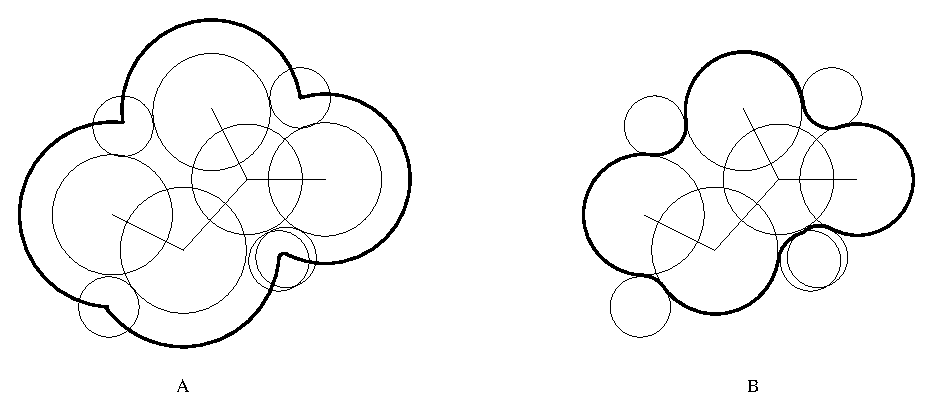
\includegraphics{cavity_types}
\par\end{centering}

\caption{\label{fig1}Different types of the molecular cavity surfaces: a)
the solvent accessible surface, b) the solvent excluding surface}
\end{figure}


The resulting cavity of atomic spheres is smoothed by adding some
more spheres not centered on atomic nuclei to approximate the solvent
excluding surface (Figure \ref{fig2}).
\begin{figure}
\begin{centering}
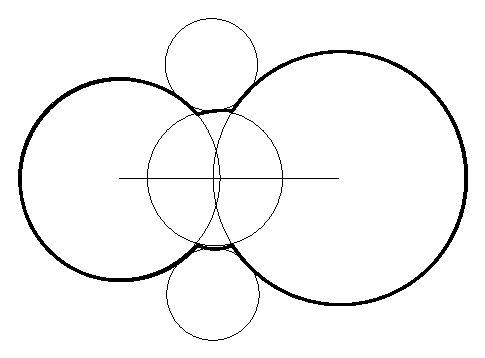
\includegraphics{aproxim}
\par\end{centering}

\caption{\label{fig2}The approximation of the solvent excluding surface by
the additional sphere}
\end{figure}


Each sphere is then subdivided into triangular tesserae corresponding
to the projections on the surface the faces of a polyhedron inscribed
in this sphere (Figure \ref{fig3}). To satisfy the symmetry of the
solute, different polyhedron types can be chosen (tetrahedron, cube,
dodecahedron and others). Tesserea completely buried by some other
spheres are discarded, while those cut by intersections with one or
more spheres are replaced by new tesserae whose areas are estimated
applying the Gauss-Bonnet theorem \cite{Cossi96}. Applying the Gauss-Bonnet
theorem give a possibility to have an analytical expression for area
of the cut tesserae and consequently to have analytical derivatives
of a surface elements of the cavity respect to nuclear coordinates
of the solute molecule.
\begin{figure}
\begin{centering}
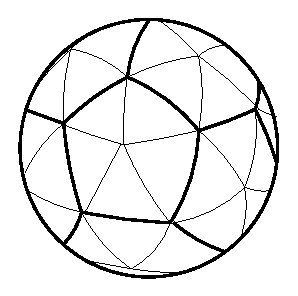
\includegraphics{project}
\par\end{centering}

\caption{\label{fig3}A schematic representation of the tessellation of a sphere
in terms of pentakisdodecahedron faces.}
\end{figure}



\section{Instabilities of the GEPOL algorithm and applying switching functions
to avoid them}

The GEPOL algorithm used to generate a molecular cavity and a set
of of representative points used in PCM calculations possesses a number
of features which very often cause instabilities during optimization
of a solute structure. 

First of all the set of additional non-atom centered spheres is not
constant value and depends on the current structure of molecule. Even
the small changing molecular geometry can result in appearing new
or disappearing old additional spheres. As result the number of representative
points and as consequence the number of surface point charges can
be dramatically changed leading to fluctuations of solvation energy
and gradients. 

Also if during geometry optimization one sphere gradually plunges
in another, the area of intersecting tessera have to reduce smoothly.
That is true for many cases but still there are exclusions. Let\textquoteright{}s
consider the specific case when one of uncut tessera vertices is located
exactly on the surface of the intersecting sphere. Now, if the tessera
is moving within the intersecting sphere, the vertex is replaced by
two vertices. The moving in backward direction does not change tessera
shape. If consider infinitesimal variation of the position of the
intersecting sphere, the moving in both directions has not to change
the position of representative points. But that is wrong assumption.
The position of a representative points sjk is defined as a mean of
tessera vertices with respect of sphere center and two very close
located vertices will give double contribution into representative
point position resulting in discontinuity of point positions with
respect to molecular geometry. There are many other specific cases.
For example, cutting procedure can divide tessera into separated part
or making hole in tessera leaving untouched its vertices.

Applying the Gauss-Bonnet formula to calculate area of tessera of
arbitrary polygon shape can also be source of instabilities. Angels
used in that equation are calculated by means vectors and dot products,
direct and inverse trigonometric functions. In the extreme cases when
angles are close to 0\textdegree{} or 180\textdegree{} eq. 2 can produces
very poor numerical results.

The simplest way to increase stability of the GEPOL algorithm is to
use atomic centered spheres only or to fix iterative procedure of
generating additional spheres to have for different molecular geometries
the same set of spheres. Unfortunately that method can produce one
more source of instabilities. Two spheres can be very close to each
other or on the contrary can be interlocked a bit. In the standard
GEPOL algorithm such situation in both cases results in generation
of one, at least, additional sphere. But that is not the case if the
fixed set of spheres is used. As result the distance between the representative
points of two tesserae on two neighboring spheres can be very short
compared to their size. This can lead to very strong interaction between
surface point charges located at those representative points and energetic
and gradient instabilities.


\subsection{Switching functions approach}

Switching functions serve to provide smooth appearance or disappearance
representative points and guaranty rigorously smooth PES for solvation
model. Generally, switching functions define appearance and disappearance
of any representative point as a smooth and continuous function $S_{jkm}\left(r_{jkm}\right)$
of distance $r_{jkm}$ between the point \textit{j} belonged sphere
\textit{k} and the other sphere \textit{m}. The total switching function
of the given representative point is the product with respect to all
spheres forming molecular SES, excluding the sphere to which the point
belongs:
\begin{equation}
S_{jk}={\textstyle {\displaystyle \prod_{m=1,m\neq j}^{N-1}S_{jkm}\left(r_{jkm}\right)}}\label{sw_f1}
\end{equation}


Algorithms using switching functions are mostly based on:
\begin{enumerate}
\item atomic centered spheres only;
\item number of the representative points are constant for any molecular
configurations;
\item tesserae are not cut by intersecting spheres but their areas are scaled
smoothly by switching functions;
\item positions of the representative points are defined exclusively by
the positions of centers of spheres they belong.
\end{enumerate}
\begin{figure}
\begin{centering}
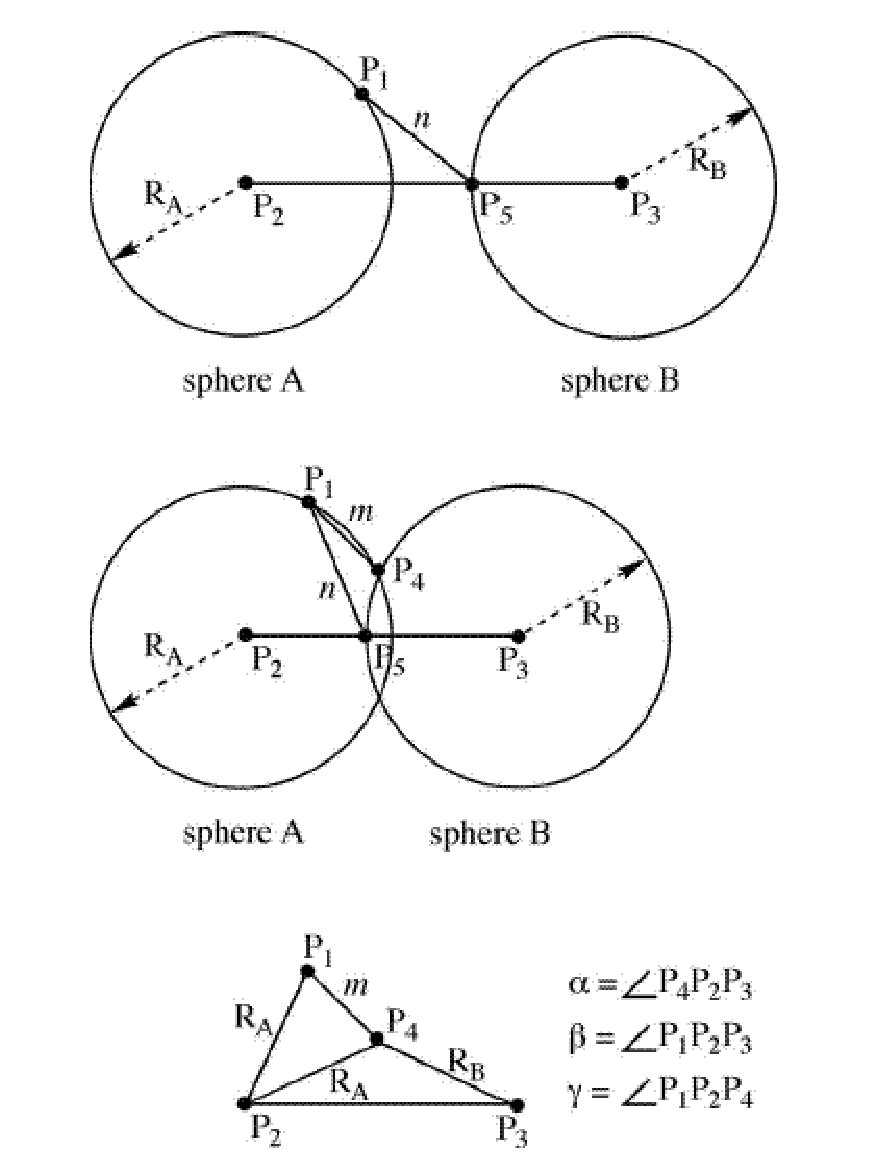
\includegraphics[scale=0.5]{fixpva}
\par\end{centering}

\caption{\label{fig10}Definition of FIXPVA scheme}
\end{figure}
Scaling tessera areas reduces electrostatic interaction of the close
located surface point charges. Removing cutting procedure stabilizes
generation of surface point grid, as the Gauss-Bonnet formula no longer
used. As the result, PES should be smooth and continuous, geometrical
gradients of representative point are very simple and stable. The
main disadvantage of tessellation schemes is that they all underestimate
the solvent excluded surface (SES). As the result, the calculated
solvation energy as rule is smaller than produced by standard GEPOL
tessellation scheme.

In ParaGauss the new smoothing scheme FIXPVA \cite{Su09} has been
implemented. The switching function in FIXPVA is defined by product
of two functions, $S_{jkm}^{1}$ and $S_{jkm}^{2}$,
\begin{equation}
S_{jkm}^{1}=\begin{cases}
\begin{array}{l}
1,\\
10\left(\frac{m^{2}-m_{1}^{2}}{m_{2}^{2}-m_{1}^{2}}\right)^{3}-15\left(\frac{m^{2}-m_{1}^{2}}{m_{2}^{2}-m_{1}^{2}}\right)^{4}+6\left(\frac{m^{2}-m_{1}^{2}}{m_{2}^{2}-m_{1}^{2}}\right)^{5}\\
0,
\end{array} & \begin{array}{l}
m>m_{2}\\
m_{2}\geq m>m_{1}\\
m_{1}\geq m
\end{array}\end{cases}\label{sw_f2}
\end{equation}
\begin{equation}
S_{jkm}^{2}=\begin{cases}
\begin{array}{l}
1,\\
10\left(\frac{n^{2}-n_{1}^{2}}{n_{2}^{2}-n_{1}^{2}}\right)^{3}-15\left(\frac{n^{2}-n_{1}^{2}}{n_{2}^{2}-n_{1}^{2}}\right)^{4}+6\left(\frac{n^{2}-n_{1}^{2}}{n_{2}^{2}-n_{1}^{2}}\right)^{5}\\
0,
\end{array} & \begin{array}{l}
n>n_{2}\\
n_{2}\geq n>n_{1}\\
n_{1}\geq n
\end{array}\end{cases}\label{sw_f3}
\end{equation}


\textit{m }is is the distance between representative point \textit{jk}
(P1) and intersecting point (P4) of other sphere. Points (P1), (P4)
and centers of two considered spheres, points (P2) and (P3), are on
the same plane. \textit{n} is the distance between representative
point \textit{jk} (P1) and surface point (P5) of other sphere on the
line connecting centers of both spheres, (P2) and (P3) (Figure \ref{fig10}):
\begin{equation}
m^{2}=\left|\overrightarrow{r}_{1}-\overrightarrow{r}_{4}\right|^{2}\label{sw_f4}
\end{equation}
\begin{equation}
n^{2}=\left|\overrightarrow{r}_{1}-\overrightarrow{r}_{5}\right|^{2}\label{sw_f5}
\end{equation}


The stability of the FIXPVA algorithm and values of calculated solvation
energies depends on parameters $m_{1,2}$ and $n_{1,2}$. For $m_{1}$
and $m_{2}$ the original values are 0.02 and 0.3 �, respectively,
and 1.0 and 1.5 � for $n_{1}$ and $n_{2}$. The parameters $m_{1,2}$
have been chosen to avoid too sharp or too wide switching functions.
$n_{1,2}$ parameters prevent too close contact of two different spheres
that can leads to strong electrostatic interaction between surface
point charges. In our implementation we apply a bit smaller parameters
$m_{1,2}$ (0.01, 0.29 �) and $n_{1,2}$ (0.53, 1.06 �) that allow
to increase the value of reproduced SES and do not reduce stability
of geometry optimization process.


\section{Continuum solvation model (electrostatic contribution) for 2-D periodic
systems}

Two dimensional periodic system is a set of unique atoms ({}``unit
cell'') replicated along two independent displacement vectors $\overrightarrow{a}_{1}$
and $\overrightarrow{a}_{2}$. Each replica of the unit cell is defined
by a vector $\overrightarrow{a}=n_{1}\overrightarrow{a}_{1}+n_{2}\overrightarrow{a}_{2}$.
The solvent reaction field will be given also by a unique set of solvation
point charges replicated along the vectors $\overrightarrow{a}_{1}$
and $\overrightarrow{a}_{2}$. The COSMO equation (eq. \ref{cosmo2})
must be generalized in order to calculate the unique solvation charges,
taking into account the interaction with all their periodic images.
The potential generated by all solvation charges in point \textit{i},
$V_{i}$, is written as a Coulomb sum
\begin{equation}
\begin{array}{cl}
V_{i}= & A_{ii}q_{i}+{\displaystyle \sum_{j\neq i}^{N}A_{ij}q_{j}+q_{i}{\displaystyle \sum_{n_{1},n_{2}=-\infty}^{+\infty}\frac{1}{\left|n_{1}\overrightarrow{a}_{1}+n_{2}\overrightarrow{a}_{2}\right|}}}\\
 & +{\displaystyle \sum_{j\neq i}^{N}}q_{j}{\displaystyle \sum_{n_{1},n_{2}=-\infty}^{+\infty}}\frac{1}{\left|\overrightarrow{r}_{ij}+n_{1}\overrightarrow{a}_{1}+n_{2}\overrightarrow{a}_{2}\right|}.
\end{array}\label{2D1}
\end{equation}


The first two terms of eq. (\ref{2D1}) are the contribution of the
unique charges; the third therm takes into account the periodic images
of the charge $q_{i}$, and the fourth term accounts for the images
of all the other charges $q_{j}$; $\overrightarrow{r}_{ij}$ is the
distance between unique solvation charges in the unit cell. Unfortunately
even if the total solvation charge is equal to zero, the last two
terms diverge with $n_{1}$and $n_{2}$. Therefore eq. (\ref{2D1})
cannot be used to calculate elements of the A matrix. 

To calculate contribution of each unique solvation charges and their
periodic images in \cite{Cossi04} the suggestion made in \cite{Takemoto03}
for the electrostatic energy of an ionic crystals was used. If consider
a lattice vector $\overrightarrow{a}=n_{1}\overrightarrow{a}_{1}+n_{2}\overrightarrow{a}_{2}$,
it define a direction, along which all images have the same ration
$\nicefrac{n_{1}}{n_{2}}$; and the two last terms of eq. (\ref{2D1})
is replaced by the sum ${\displaystyle \sum_{\overrightarrow{a}}V_{i}^{\overrightarrow{a}}}$
and

\begin{equation}
V_{i}^{\overrightarrow{a}}=2q_{i}{\displaystyle \sum_{n=1}^{+\infty}}\frac{1}{n\left|\overrightarrow{a}\right|}+{\displaystyle \sum_{j\neq i}^{N}}q_{j}{\displaystyle \sum_{n=1}^{+\infty}}\left(\frac{1}{\left|\overrightarrow{r}_{ij}+n\overrightarrow{a}\right|}+\frac{1}{\left|\overrightarrow{r}_{ij}-n\overrightarrow{a}\right|}\right).\label{2D2}
\end{equation}


The last sum can be rewritten using Legendre polynomials. Then
\begin{equation}
\begin{array}{cll}
\frac{1}{\left|\overrightarrow{r}_{ij}+n\overrightarrow{a}\right|} & = & \frac{1}{n\left|\overrightarrow{a}\right|}{\displaystyle \sum_{m=0}^{+\infty}}\left(\frac{\left|\overrightarrow{r}_{ij}\right|}{\left|n\overrightarrow{a}\right|}\right)^{m}P_{m}\left(\cos\theta_{ij}^{\overrightarrow{a}}\right)\\
 & = & \frac{1}{n\left|\overrightarrow{a}\right|}+\frac{1}{\left|\overrightarrow{a}\right|}{\displaystyle \sum_{m=1}^{+\infty}}\left(\frac{\left|\overrightarrow{r}_{ij}\right|}{\left|\overrightarrow{a}\right|}\right)^{m}\frac{1}{\left|n\right|^{m+1}}P_{m}\left(\cos\theta_{ij}^{\overrightarrow{a}}\right).
\end{array}\label{2D3}
\end{equation}


Here $P_{m}$ is the polynomial of order $m$, and $\theta_{ij}^{\overrightarrow{a}}$is
the angle between $\overrightarrow{r}_{ij}$ and the vector $\overrightarrow{a}$
\begin{figure}
\begin{centering}
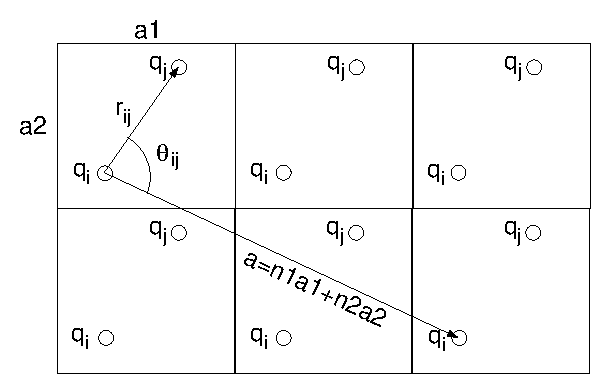
\includegraphics[scale=0.8]{slab}
\par\end{centering}

\caption{\label{fig11}The set of unique solvation charges replicated along
vector $\protect\overrightarrow{a}=n_{1}\protect\overrightarrow{a}_{1}+n_{2}\protect\overrightarrow{a}_{2}$
with $n_{1}=1$and $n_{2}=2$}
\end{figure}
 (Figure \ref{fig11}). For $n\rightarrow-n$, the only change is
$\cos\theta_{ij}^{\overrightarrow{a}}\rightarrow-\cos\theta_{ij}^{\overrightarrow{a}}$.
It allows to cancel out the odd terms in eq. (\ref{2D2}), leaving
\begin{equation}
\begin{array}{cl}
V_{i}^{\overrightarrow{a}}= & 2q_{i}{\displaystyle \sum_{n=1}^{+\infty}}\frac{1}{n\left|\overrightarrow{a}\right|}+{\displaystyle \sum_{j\neq i}^{N}}q_{j}\left[2{\displaystyle \sum_{n=1}^{+\infty}}\frac{1}{n\left|\overrightarrow{a}\right|}\right.\\
 & \left.+\frac{2}{\left|\overrightarrow{a}\right|}{\displaystyle \sum_{m=1}^{+\infty}}\left(\frac{\left|\overrightarrow{r}_{ij}\right|}{\left|\overrightarrow{a}\right|}\right)^{2m}\varsigma\left(2m+1\right)P_{2m}\left(\cos\theta_{ij}^{\overrightarrow{a}}\right)\right].
\end{array}\label{2D4}
\end{equation}


Here the Riemann $\varsigma$-function was introduced:
\begin{equation}
\varsigma\left(x\right)={\displaystyle \sum_{n=1}^{+\infty}}\frac{1}{n^{x}}.\label{2D5}
\end{equation}


If the total solvation charge is equal to zero, i.e., $q_{i}+\sum_{j\neq i}q_{j}=0$,
all diverging terms in eq. (\ref{2D4}) disappear. The final equation
for 2-D periodic set of solvation charges is written as
\begin{equation}
\begin{array}{cl}
V_{i}^{\overrightarrow{a}}= & {\displaystyle \sum_{j\neq i}^{N}}\left[{\displaystyle \sum_{n_{1},n_{2}}\frac{2}{\left|n_{1}\overrightarrow{a}_{1}+n_{2}\overrightarrow{a}_{2}\right|}}\right.\\
 & \left.\times{\displaystyle \sum_{m=1}^{+\infty}}\left(\frac{\left|\overrightarrow{r}_{ij}\right|}{\left|n_{1}\overrightarrow{a}_{1}+n_{2}\overrightarrow{a}_{2}\right|}\right)^{2m}\varsigma\left(2m+1\right)P_{2m}\left(\cos\theta_{ij}^{\overrightarrow{a}}\right)\right]={\displaystyle \sum_{j\neq i}^{N}}V_{ij}^{\overrightarrow{a}}.
\end{array}\label{2D6}
\end{equation}


To avoid over-counting on the same line the greatest common divisor
of the set $\left(n_{1},n_{2}\right)$ should be unity, and $n_{1}$
should be a positive integer and $n_{2}$ an integer. Of course, the
case $n_{1}=0,\: n_{2}=0$ has to be excluded.

Quantum mechanical program exploiting plane-wave basis sets operate
exclusively with 3D periodicity. In this case according to \cite{Takemoto03}
the coupling term depended on shape of the unit cell has to be added:
\begin{equation}
\begin{array}{cl}
V_{i}^{\overrightarrow{a}}= & {\displaystyle \sum_{j\neq i}^{N}}\left[{\displaystyle \sum_{n_{1},n_{2},n_{3}}\frac{2}{\left|n_{1}\overrightarrow{a}_{1}+n_{2}\overrightarrow{a}_{2}+n_{3}\overrightarrow{a}_{3}\right|}}\right.\\
 & \left.\times{\displaystyle \sum_{m=1}^{+\infty}}\left(\frac{\left|\overrightarrow{r}_{ij}\right|}{\left|n_{1}\overrightarrow{a}_{1}+n_{2}\overrightarrow{a}_{2}+n_{3}\overrightarrow{a}_{3}\right|}\right)^{2m}\varsigma\left(2m+1\right)P_{2m}\left(\cos\theta_{ij}^{\overrightarrow{a}}\right)+\left|\overrightarrow{r}_{ij}\right|^{2}\right]={\displaystyle \sum_{j\neq i}^{N}}V_{ij}^{\overrightarrow{a}}.
\end{array}\label{2D7}
\end{equation}


Here he greatest common divisor of the set $\left(n_{1},n_{2},n_{3}\right)$
should be unity, and one of three integers should be positive.

Now we can rewrite elements of the COSMO matrix \textbf{A} for periodic
solute in the form:
\begin{equation}
\begin{cases}
A_{ii}^{2D}= & A_{ii}\\
A_{ij}^{2D}= & A_{ij}+V_{ij}^{\overrightarrow{a}}
\end{cases}\label{2D8}
\end{equation}



\section{Dispersion and Repulsion energies: pair-potential model}

The calculation of the dispersion and repulsion contribution to the
free solvation energy of the solute is based on an atom-atom pair
potential method \cite{Pertsin86,Claverie78}. In frameworks of this
method the dispersion and short-range repulsion interactions between
solute and solvent molecules are presented by means of a Buchingham
formula 
\begin{equation}
V_{ij}=K_{ij}\left[-\frac{A}{z_{ij}^{6}}+C\exp(-\alpha z_{ij})\right]\label{disp1}
\end{equation}
 where 
\begin{equation}
z_{ij}=r_{ij}/R_{ij}^{0}\label{disp2}
\end{equation}
 $A=-0.214$, $C=47000$ (corresponding to $V_{ij}$ expressed in
kcal/mol) and $\alpha=12.35$ do not depend on the solute ($i$) and
solvent ($j$) atoms involved, $r_{ij}$ is distance between the solute
and solvent atoms. Thus one only needs to determine the two parameters
$K_{ij}$ and $R_{ij}^{0}$ for each pair of atoms ($i,j$). In \cite{Claverie78}
they were expressed in terms of atomic parameters $k_{l}$ and $R_{l}^{W}$:
\begin{equation}
R_{ij}^{0}=\sqrt{(2R_{i}^{W})(2R_{j}^{W})}\label{disp3}
\end{equation}
 
\begin{equation}
K_{ij}=k_{i}k_{j}\label{disp5}
\end{equation}


The procedure to determine pair parameters $K_{ij}$ and $R_{ij}^{0}$
is typically nontrivial\cite{Claverie78}, but parameters $R_{l}^{W}$
are very close to van der Waals radii of individual atoms (Bondi radii,
for example \cite{Bondi64}) and very often those values are used
in practical calculations \cite{Claverie87,Claverie76,Claverie81}.

Using the pair-potential method described above, the procedure of
computing the dispersion-repulsion interaction between a solute and
a continuum solvent has been suggested in \cite{Floris91}. In this
paper the two-body function like eq. \ref{disp1} has been used 
\begin{equation}
V_{ij}(r_{ij})=-\frac{d_{ij}}{r_{ij}^{6}}+c_{ij}\exp(-\gamma_{ij}r_{ij})\label{disp4}
\end{equation}
 where parameters $d_{ij}$, $c_{ij}$ and $\gamma_{ij}$ can be found
by means $k_{l}$ and $R_{l}^{W}$atomic parameters.

To obtain the solute-solvent dispersion-repulsion energy one needs
to know the distribution of the solvent molecules around the solute
molecule. In the frame of the continuum solvation model this distribution
may be written in the following form 
\begin{equation}
\sigma_{ij}\left(\overrightarrow{r_{ij}}\right)=\rho_{s}g_{ij}\left(\overrightarrow{r}_{ij}\right)\label{disp6}
\end{equation}
 Here $\rho_{s}$ is the number density of the solvent molecules and
$g_{ij}\left(\overrightarrow{r}_{ij}\right)$ is a correlation function,
depending on the position of $j$ in respect to $i$.

The dispersion-repulsion contribution to the free solvation energy
may by written as a sum of volume integrals: 
\begin{eqnarray}
G_{d-r} & = & \sum_{ij}\int\sigma_{ij}\left(\overrightarrow{r}_{ij}\right)V_{ij}(r_{ij})d\overrightarrow{r}_{ij}\nonumber \\
 & = & \rho_{s}\sum_{ij}\left[-d_{ij}\int\frac{g_{ij}\left(\overrightarrow{r}_{ij}\right)}{r_{ij}^{6}}d\overrightarrow{r}_{ij}+c_{ij}\int g_{ij}\left(\overrightarrow{r}_{ij}\right)\exp(-\gamma_{ij}r_{ij})d\overrightarrow{r}_{ij}\right]\label{disp7}
\end{eqnarray}
 The integrals in eq. (\ref{disp7}) are defined over the entire space,
but the presence of short range repulsions allows to define a portion
of the space, containing the solute molecule, in which there are no
atoms $j$ of the solvent molecules. In other words, one can introduce
for each $j$ a closed volume $C_{j}$ so that 
\begin{equation}
g_{ij}\left(\overrightarrow{r}_{ij}\right)=0,\: if\:\overrightarrow{r}_{ij}\in C_{j}\label{disp8}
\end{equation}


On the basis of this consideration in \cite{Floris91} the approximate
model, which assumes the existence of $C_{l}$ cavities and uses simple
analytical expression of the correlation function $g_{ij}\left(\overrightarrow{r}_{ij}\right)$,
has been developed.

The cavity suitable for the calculation of dispersion-repulsion terms
is different from that used to calculate the electrostatic term. Since
the atomic pair-potential used (eq. \ref{disp4}) depends on the distances
between the nuclei, it is appropriate to define the cavity as the
portion of space from which the nuclei of the solvent atoms are excluded.
For each solvent atom one defines a new cavity $C_{l}$ described
with a set of spheres centered on the solute atoms\cite{Cossi96}.
In this case the radii of the spheres are augmented by the radius
of the solvent atom. These cavity surfaces correspond to the solvent
accessible surface (Figure \ref{fig4}).
\begin{figure}
\begin{centering}
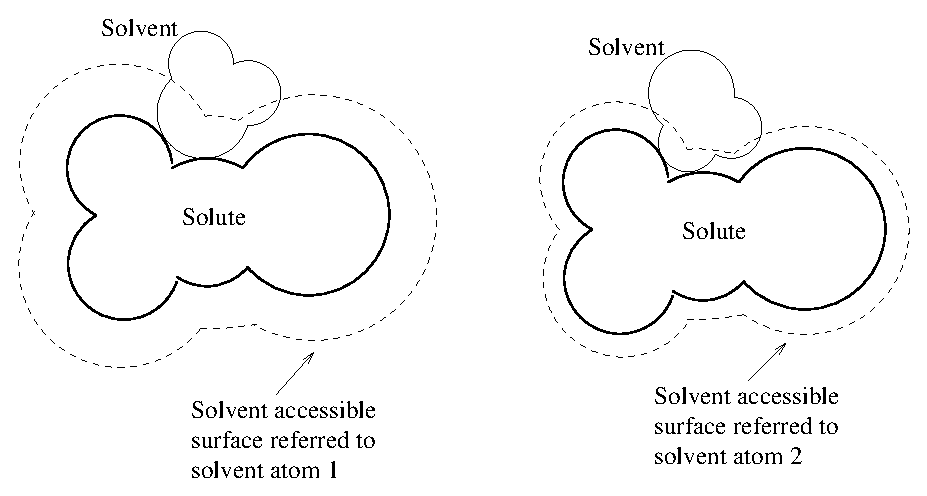
\includegraphics{acces_surf}
\par\end{centering}

\caption{\label{fig4}Definition of solvent accessible surfaces referred to
solvent atoms}
\end{figure}


There are different approximations of $g_{ij}\left(\overrightarrow{r}_{ij}\right)$
depending on the solvent properties. A very useful approximation is
the simplest one

\begin{equation}
g_{ij}(\overrightarrow{r}_{ij})=\left\{ \begin{array}{c}
0,\: if\:\overrightarrow{r}_{ij}\in C_{j}\\
1,\: if\:\overrightarrow{r}_{ij}\notin C_{j}
\end{array}\right.\label{disp9}
\end{equation}
 corresponding to homogeneous distribution of the solvent ( $homogeneous$
$approximation$ \cite{Floris91}). When the integrals of eq. \ref{cav7}
are limited to the portion of space outside $C_{l}$ cavity, they
can be transformed into surface integrals, computed on the $\Sigma_{j}$
surface. This has been done in \cite{Floris91}. The resulting expression
can be written in the following form 
\begin{eqnarray}
G_{d-r} & = & \rho_{s}\sum_{ij}\left[\int_{\Sigma_{l}}A_{ij}^{d}(r_{ij})\overrightarrow{r}_{ij}\right.\nonumber \\
 & \cdot & \left.\widehat{n_{\Sigma_{l}}}ds+\int_{\Sigma_{l}}A_{ij}^{r}(r_{ij})\overrightarrow{r}_{ij}\widehat{n}_{\Sigma_{l}}ds\right]\label{disp10}
\end{eqnarray}


The integrals of eq. (\ref{disp10}) can be calculated numerically.
The surface of cavity $C_{l}$ is replaced by set of tesserae with
area $s_{k}$ and then the eq. (\ref{disp10}) is replaced by the
sum 
\begin{eqnarray}
G_{d-r} & = & \rho_{s}\sum_{ij}\sum_{k}\nonumber \\
 &  & \left[A_{ij}^{d}(r_{ij})+A_{ij}^{r}(r_{ij})\right]\overrightarrow{r}_{ij}\widehat{n}_{k}s_{k}\label{disp11}
\end{eqnarray}
 where $\widehat{n}_{k}$ is the versor normal to the cavity $C_{l}$
in the center of tessera $k$. The terms $A_{ij}^{d}(r_{ij})$ and
$A_{ij}^{r}(r_{ij})$ in eqs. (\ref{disp10} and \ref{disp11}) are
\begin{equation}
A_{ij}^{d}(r_{ij})=-\frac{d_{ij}}{3r_{ij}^{6}}\label{disp12}
\end{equation}
 
\begin{equation}
A_{ij}^{r}(r_{ij})=c_{ij}\exp(-\gamma_{ij}r_{ij})\left[\frac{1}{\gamma_{ij}r_{ij}}+\frac{2}{(\gamma_{ij}r_{ij})^{2}}+\frac{2}{(\gamma_{ij}r_{ij})^{3}}\right]\label{disp14}
\end{equation}
 The derivatives of $G_{d-r}$ with respect to the atomic coordinates
of the solute are
\begin{eqnarray}
G_{d-r}^{x} & = & \rho_{s}\sum_{ij}\sum_{k}\left\{ \left[A_{ij}^{d}(r_{ij})+A_{ij}^{r}(r_{ij})\right]^{x}\overrightarrow{r}_{ij}\widehat{n}_{k}s_{k}+\left[A_{ij}^{d}(r_{ij})+A_{ij}^{r}(r_{ij})\right]\overrightarrow{r}_{ij}^{x}\widehat{n}_{k}s_{k}\right.\nonumber \\
 & + & \left.\left[A_{ij}^{d}(r_{ij})+A_{ij}^{r}(r_{ij})\right]\overrightarrow{r}_{ij}\widehat{n}_{k}^{x}s_{k}+\left[A_{ij}^{d}(r_{ij})+A_{ij}^{r}(r_{ij})\right]\overrightarrow{r}_{ij}\widehat{n}_{k}s_{k}^{x}\right\} \label{disp13}
\end{eqnarray}
 and
\begin{eqnarray}
G_{d-r}^{x} & = & \rho_{s}\sum_{ij}\sum_{k}\left\{ \left[A_{ij}^{d}(r_{ij})+A_{ij}^{r}(r_{ij})\right]^{xy}\overrightarrow{r}_{ij}\widehat{n}_{k}s_{k}+\left[A_{ij}^{d}(r_{ij})+A_{ij}^{r}(r_{ij})\right]^{x}\overrightarrow{r}_{ij}^{y}\widehat{n}_{k}s_{k}\right.\nonumber \\
 & + & \left[A_{ij}^{d}(r_{ij})+A_{ij}^{r}(r_{ij})\right]^{x}\overrightarrow{r}_{ij}\widehat{n}_{k}^{y}s_{k}+\left[A_{ij}^{d}(r_{ij})+A_{ij}^{r}(r_{ij})\right]^{x}\overrightarrow{r}_{ij}\widehat{n}_{k}s_{k}^{y}\nonumber \\
 & + & \left[A_{ij}^{d}(r_{ij})+A_{ij}^{r}(r_{ij})\right]^{y}\overrightarrow{r}_{ij}^{x}\widehat{n}_{k}s_{k}+\left[A_{ij}^{d}(r_{ij})+A_{ij}^{r}(r_{ij})\right]\overrightarrow{r}_{ij}^{xy}\widehat{n}_{k}s_{k}\nonumber \\
 & + & \left[A_{ij}^{d}(r_{ij})+A_{ij}^{r}(r_{ij})\right]\overrightarrow{r}_{ij}^{x}\widehat{n}_{k}^{y}s_{k}+\left[A_{ij}^{d}(r_{ij})+A_{ij}^{r}(r_{ij})\right]\overrightarrow{r}_{ij}^{x}\widehat{n}_{k}s_{k}^{y}\nonumber \\
 & + & \left[A_{ij}^{d}(r_{ij})+A_{ij}^{r}(r_{ij})\right]^{y}\overrightarrow{r}_{ij}\widehat{n}_{k}^{x}s_{k}+\left[A_{ij}^{d}(r_{ij})+A_{ij}^{r}(r_{ij})\right]\overrightarrow{r}_{ij}^{y}\widehat{n}_{k}^{x}s_{k}\nonumber \\
 & + & \left[A_{ij}^{d}(r_{ij})+A_{ij}^{r}(r_{ij})\right]\overrightarrow{r}_{ij}\widehat{n}_{k}^{xy}s_{k}+\left[A_{ij}^{d}(r_{ij})+A_{ij}^{r}(r_{ij})\right]\overrightarrow{r}_{ij}\widehat{n}_{k}^{x}s_{k}^{y}\nonumber \\
 & + & \left[A_{ij}^{d}(r_{ij})+A_{ij}^{r}(r_{ij})\right]^{y}\overrightarrow{r}_{ij}\widehat{n}_{k}s_{k}^{x}+\left[A_{ij}^{d}(r_{ij})+A_{ij}^{r}(r_{ij})\right]\overrightarrow{r}_{ij}^{y}\widehat{n}_{k}s_{k}^{x}\nonumber \\
 & + & \left.\left[A_{ij}^{d}(r_{ij})+A_{ij}^{r}(r_{ij})\right]\overrightarrow{r}_{ij}\widehat{n}_{k}^{y}s_{k}^{x}+\left[A_{ij}^{d}(r_{ij})+A_{ij}^{r}(r_{ij})\right]\overrightarrow{r}_{ij}\widehat{n}_{k}s_{k}^{xy}\right\} \label{disp15}
\end{eqnarray}



\section{Cavitation energy}

The calculation of the cavitation energy is based on the scaled particle
theory of fluids developed by R. A. Pierotti \cite{Pierroti76}. The
essence of the scaled particle theory is to require that the centers
of solvent molecules are excluded from a given region of space in
the solvent. This theory assumes a fluid of spherically symmetrical
hard core molecules with diameter $\sigma_{1}$. A cavity in solvent
can be created by excluding the centers of all \textit{N} solvent
molecules from a spherical region of space of radius \textit{r} in
the total volume \textit{V} of the solvent. The probability that such
a cavity exists is $p_{0}(r,\rho)$, where $\rho$ is the number density
of solvent ($N/V$). The cavity could be created as result of a statistical
fluctuation, and the probability of such fluctuation is \cite{Kirkw68}

\begin{equation}
p_{0}(r,\rho)=e^{-W(r,\rho)/kT}\label{cav1}
\end{equation}
 where $W(r,\rho)$ is the reversible work to produce a cavity of
radius $r$ in the solvent. The scaled particle theory attempts to
determine $p_{0}(r,\rho)$ as accurately as possible using statistical
mechanics and geometrical arguments. The general approach is to start
with a cavity of zero radius and allow its to grow up to the desired
radius (Figure \ref{fig5}).
\begin{figure}
\begin{centering}
\includegraphics{cav_en_1}
\par\end{centering}

\caption{\label{fig5}Spherical cavity of radius \textit{r} caused by a hard-sphere
solute of diameter $\sigma_{2}$ in hard-sphere solvent of molecules
of diameter $\sigma_{1}$.}
\end{figure}


To consider the probability of finding a molecular center just outside
the cavity of radius $r$ one should calculate the probability of
finding the center in the solvent shell of thickness $r$ to $r+dr$.
This probability is given by $4\pi r^{2}\rho G(r,\rho)dr$, where
$G(r,\rho)$ is conditional probability that molecular center is located
in that region. The probability that there is no center in this spherical
shell is simply $1-4\pi r^{2}G(r,\rho)dr$.

The probability that there is no molecular center in range $r$ to
$r+dr$ is 
\begin{equation}
p_{0}(r+dr)=p_{0}(r)+\left(\frac{\partial p_{0}(r)}{\partial r}\right)dr=p_{0}(r)\left[1-4\pi r^{2}\rho G(r,\rho)dr\right]\label{cav2}
\end{equation}
 or 
\begin{equation}
\left(\frac{\partial\ln p_{0}(r)}{\partial r}\right)=-4\pi r^{2}\rho G(r,\rho)\label{cav3}
\end{equation}
 Using eq. (\ref{cav1}), we find 
\begin{equation}
\left(\partial W(r,\rho)/kT/dr\right)=4\pi r^{2}\rho G(r,\rho)\label{cav4}
\end{equation}
 and consequently 
\begin{equation}
W(r,\rho)/kT=4\pi\rho\int_{0}^{r}r^{2}G(r,\rho)dr\label{cav5}
\end{equation}


To define the reversible work of building a cavity in a solvent one
has to determine a functional representation of the conditional probability
$G(r,\rho)$. The very suitable representation is an asymptotic expansion
in $1/r$\cite{Tully71}. In this case one can write that
\begin{equation}
G(r,\rho)=\sum_{i}G_{i}(r,\rho)(1/r)^{i}\label{cav6}
\end{equation}


For all values of $r\leq\sigma_{1}/2$, one and only one hard-core
molecule of a solvent can have its center in the spherical cavity
of radius $r$, otherwise the hard core would have to overlap. The
probability that a molecular center is in this region is $\frac{4}{3}\pi r^{3}\rho$,
hence 
\begin{equation}
p_{0}=1-\frac{4}{3}\pi r^{3}\rho\qquad r\leq\sigma_{1}/2\label{cav7}
\end{equation}
 Reference to eq. (\ref{cav3}) indicates that 
\begin{equation}
G(r,\rho)=\frac{1}{(1-\frac{4}{3}\pi r^{3}\rho)}\qquad r\leq\sigma_{1}/2\label{cav8}
\end{equation}
 Inserting eq. (\ref{cav8}) into eq. (\ref{cav5}) and carrying out
the integration one can write 
\begin{equation}
W_{0}(r,\rho)=kT\ln(1-\frac{4}{3}\pi r^{3}\rho)\qquad r\leq\sigma_{1}/2\label{cav10}
\end{equation}
 where $W_{0}(r,\rho)$ is the reversible work to produce a cavity
of radius $r\leq\sigma_{1}/2$.

There are a host exact conditions that can be found in additional
to that of eq. (\ref{cav8}). They have led to the evaluation of $G_{i}$
in eq. (\ref{cav6}) through $G_{5}$ \cite{Tully71}. It has been
shown that $G_{3}$ is equal zero and $G_{4}$ is likely to be zero.
Examination of eqs. (\ref{cav5} and \ref{cav6}) shows that an asymptotic
expansion for $W(r,\rho)$ of form 
\begin{equation}
W(r,\rho)=K_{0}+K_{1}r+K_{2}r^{2}+K_{3}r^{3}\label{cav9}
\end{equation}
 might be an excellent approximation. This approximation incidentally
is the same form as required in classical thermodynamics 
\begin{equation}
W(r)=\frac{4}{3}\pi r^{3}P+4\pi r^{2}\gamma(1-\frac{4\delta}{r})\label{cav11}
\end{equation}
 where the term involving $P$ (the pressure) is just the volume work;
the term involving $\gamma$ (the surface tension) is the surface
work and the term involving $\frac{\delta}{r}$ corrects the surface
tension for the effect of surface curvature. In the thermodynamic
eq. \ref{cav11} the constant term $K_{0}$ is absent. For macroscopic
cavities described by eq. (\ref{cav11}), the absence of $K_{0}$
introduced negligible error but for microscopic cavities $K_{0}$
is very important term. In the original development of the scaled
particle theory, The $K$'s were obtained by expanding $W(r,\rho)$
about $r=\sigma_{1}/2$ giving 
\begin{equation}
W(r,\rho)=W_{0}+W_{0}\prime(r-\sigma_{1}/2)+\frac{1}{2}W_{0}\prime\prime(r-\sigma_{1}/2)^{2}+\frac{1}{6}W_{0}\prime\prime\prime(r-\sigma_{1}/2)^{3}\label{cav12}
\end{equation}
 where $W_{0}=kT\ln(1-\pi\sigma_{1}^{3}\rho/6)$ and where the first
and second derivatives are obtained from eq. (\ref{cav10}). The $K_{3}$
is obtained by direct comparison with thermodynamic eq. (\ref{cav11})
and hence is equal to $\frac{4}{3}\pi P$. After suitable algebraic
manipulations one can write 
\begin{equation}
\frac{W(R,\rho)}{kT}=-\ln(1-y)+\left(\frac{3y}{1-y}\right)R+\left[\frac{3y}{1-y}+\frac{9}{2}\left(\frac{y}{1-y}\right)^{2}\right]R^{2}+\frac{yP}{\rho kT}\label{cav13}
\end{equation}
 where $y=\pi\rho\sigma_{1}^{3}/6$ is the reduced number density,
$R=\sigma_{2}/\sigma_{1}$, and $\sigma_{2}$ is the diameter of the
hard-sphere solute molecule such that the cavity radius is $(\sigma_{1}+\sigma_{2})/2$.

The presented scaled particle theory was developed in \cite{Pierroti76}
for solute molecules considered as a single hard sphere. Within the
solvation model adopted for the cavity of the molecular shape (the
cavity consisted of some overlapping spheres centered on solute atoms)
\cite{Claver88}, each atomic sphere of solute of $r_{i}$ is taken
as contributing a fraction of $W(r_{i},\rho)$ proportional to its
area $A_{i}$ not buried by other spheres, so that total contribution
of the cavitation energy to the free solvation energy is 
\begin{equation}
\Delta G_{cav}=\sum_{i}\frac{A_{i}}{4\pi r_{i}^{2}}W(r_{i},\rho)\label{cav14}
\end{equation}
 The first and second derivatives of the $\Delta G_{cav}$are very
easy obtained from eq. (\ref{cav14}):
\begin{equation}
\Delta G_{cav}^{x}=\sum_{i}\frac{A_{i}^{x}}{4\pi r_{i}^{2}}W(r_{i},\rho)\label{cav15}
\end{equation}
 and
\begin{equation}
\Delta G_{cav}^{xy}=\sum_{i}\frac{A_{i}^{xy}}{4\pi r_{i}^{2}}W(r_{i},\rho)\label{cav16}
\end{equation}

\begin{thebibliography}{References}
\bibitem{Cramer95}C. J. Cramer and D. G. Truhlar, in D. G. Boyd,
K. B. Lipkowitz (Eds.), Review on computational Chemistry, V. 6, VCH,
New York, 1995 

\bibitem{Tomasi99}J. Tomasi, B. Mennucci and E. Cances, J. Mol. Structure
(Theochem), V. 464, P. 211 (1999) 

\bibitem{Miertus81}S. Miertus, E. Scrocco and J. Tomasi, Chem. Phys.,
V. 55, P. 117 (1981) 

\bibitem{Mennucci95}B. Mennucci, M. Cossi and J. Tomasi, J. Chem.
Phys., V. 102, P. 6837 (1995) 

\bibitem{Cossi94}M. Cossi, B. Mennucci and J. Tomasi, Chem. Phys.
Lett., V. 228, P. 165 (1994) 

\bibitem{Floris91}F. M. Floris, J. Tomasi and J. L. Pascual Ahuir,
J. Comp. Chem., V. 12, P. 784 (1991) 

\bibitem{Amovili94}C. Amovili, Chem. Phys. Lett., V. 229, P. 244
(1994) 

\bibitem{Amovili97}C. Amovili and B. Mennucci, J. Phys. Chem. B,
V. 101, P. 1051 (1997) 

\bibitem{Cammi94}R. Cammi and J. Tomasi, J. Chem. Phys., V. 100,
P. 7495 (1994) 

\bibitem{Cammi94a}R. Cammi and J. Tomasi, J. Chem. Phys., V. 101,
P. 3888 (1994) 

\bibitem{Klamt93}A. Klamt and G. Sch��rman, J. Chem. Soc., Perkins
Trans. 2, P. 799 (1993) 

\bibitem{Stefan95}T. N. Truong and E. V. Stefanovich, Chem. Phys.
Lett., V. 240, P. 253 (1995) 

\bibitem{Klamt95}J. Andzelm, C. K�lmel and A. Klamt, J. Chem. Phys.,
V. 103, P. 9312 (1995) 

\bibitem{Barone98}V. Barone and M. Cossi, J. Phys. Chem. A, V. 102,
P. 1995 (1998) 

\bibitem{Ben-Naim87}A. Ben-Naim, Solvation Thermodinamics, PlenumPress,
New York, 1987 

\bibitem{Tomasi94}J. Tomasi and M. Persico , Chem. Rev., V. 94, P.
2027 (1994) 

\bibitem{Cossi95}M. Cossi, J. Tomasi and R. Cammi, Int. J. Quantum
Chem.: Quantum Chem. Symp., V. 29, P. 695 (1995) 

\bibitem{Amovili99}C. Amovili, V. Barone, R. Cammi, E. Cances, M.
Cossi, B. Mennucci, C.S. Pomelli and J. Tomasi, Adv. Quantum Chem.,
V. 32, P. 227 (1999) 

\bibitem{Lee71}B. Lee and F. M. Richards, J. Mol. Biol., 55, 379
(1971) 

\bibitem{Richards77}F. M. Richards, Ann. Rev. Biophys. Bioeng., V.
6, P. 151 (1977) 

\bibitem{Pascual90}J. L. Pascual-Ahuir and E. Silla, J. Comp. Chem.,
V. 11, P. 1047 (1990) 

\bibitem{Cossi96}M. Cossi, B. Mennucci and R. Cammi, J. Comp. Chem.,
V. 17, P. 57 (1996) 

\bibitem{Cammi96}R. Cammi, M. Cossi, B. Mennucci, C. S. Pomelli and
J. Tomasi, Int. J. Quantum Chem., V. 60, P. 1165 (1996) 

\bibitem{Pertsin86}A. J. Pertsin and A. I. Kitaigorodsky, The Atom-Atom
Potential Method, Springer-Verlag, Berlin, 1986 

\bibitem{Claverie78}J. Caillet, P. Claverie and A. Pullman, Acta
Cryst., V. B34, P. 3266 (1978) 

\bibitem{Bondi64}A. Bondi, J. Phys. Chem., V. 68, P. 441 (1964) 

\bibitem{Claverie87}F. Vign�-Maeder and P. Claverie, J. Am. Chem.
Soc., V. 109, P. 24 (1987) 

\bibitem{Claverie76}J. Caillet, P. Claverie and A. Pullman, Acta
Cryst., V. B32, P. 2740 (1976) 

\bibitem{Claverie81}J. Langlet, P. Claverie, F. Caron and J. C. Boeuve,
Int. J. Quant. Chem., V. 19, P. 299 (1981) 

\bibitem{Pierroti76}R. A. Pierotti, Chem. Rev., V. 76, P. 717 (1976) 

\bibitem{Kirkw68}J. G. Kirkwood, {}``Theory of Solutions'', Gordon
and Breach, N. Y., 1968 

\bibitem{Tully71}D. M. Tully-Smith and H. Reiss, J. Chem. Phys.,
V. 53, P. 4015 (1971) 

\bibitem{Claver88}J. Langlet, P. Claverie, J. Caillet and A. Pullman,
J. Chem. Phys., V. 92, P. 1617 (1988) 

\bibitem{Su09}P. Su, H. Li, J. Chem. Phys., V. 130 074109 (2009)

\bibitem{Cossi04}M. Cossi, Chem. Phys. Letters, V. 384, P. 179 (2004) 

\bibitem{Takemoto03}H. Takemoto, T. Ohyama, A. Tohsaki, Progr. Theoret.
Phys., V. 109, P. 563 (2003) \end{thebibliography}

\end{document}
